% !TEX root = ./CSCE-636 - Homework 1 - Brody Jordan.tex

\documentclass[11pt]{article}

\usepackage[
    assignmentDueDate={September 17, 2025 at 11:59 pm}
]{C:/Users/bljor/Sync/Courses/assignment}

\PassOptionsToPackage{hyphens}{url}\usepackage{hyperref}
\usepackage{pgfplots}
\usepackage[labelfont=bf]{caption}

\begin{document}
\makeAssignmentTitle

\begin{homeworkProblem}
    Check out the Jupyter notebook for Chapter 2 at \url{https://github.com/fchollet/deep-learning-with-python-notebooks/blob/master/chapter02_mathematical-building-blocks.ipynb}. \\

    Then: \\

    For the neural network in the Jupiter notebook for the MNIST task (which has 2 layers, where the first layer has
    512 neurons and the second layer has 10 neurons), adjust the size of the first layer (namely, the number of neurons
    in the first layer) as: 16, 32, 64, 128, 256, 512. For each size, train the neural network and record its test
    accuracy (namely, accuracy on the test set). Draw a figure, where the x-axis is the size of the first layer, and the
    y-axis is the test accuracy. Submit your figure. \\

    \solution

    I completed this assignment using Google Colab. My assignment is provided here for your reference: \url{https://colab.research.google.com/drive/15D1XJKpvRMuAdVwE2G9n1ysf3vmLAD1Z}. \\

    I varied the number of neurons in the first layer of the neural network and observed the resulting model accuracy. For each iteration of the model, I used an epoch of 5, and a batch size of 128. My findings are shown below

    \begin{figure}[h!]
        \vspace{0.5\baselineskip}
        \centering
        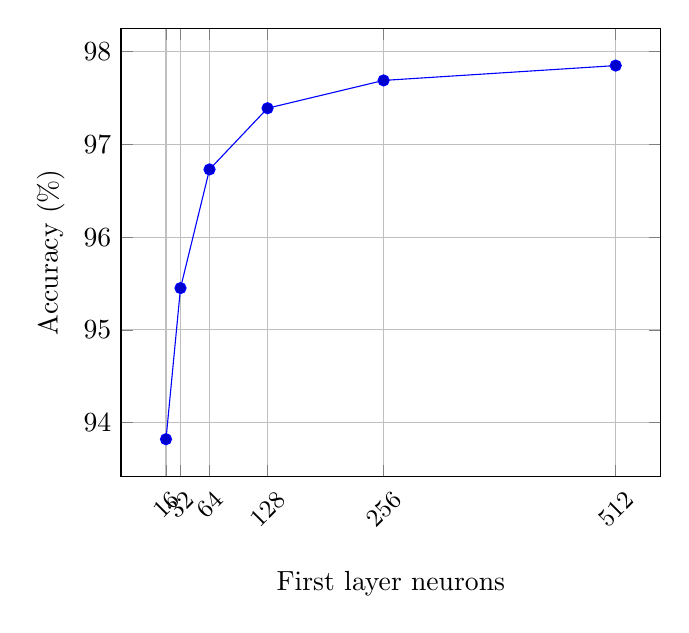
\begin{tikzpicture}

            \begin{axis}[
                    xlabel=First layer neurons,
                    ylabel=Accuracy (\%),
                    xtick={16, 32, 64, 128, 256, 512},
                    xticklabel style={rotate=45, font=\small},
                    xlabel style={yshift=-0.25cm},
                    grid=major
                ]
                \addplot coordinates {
                        (16, 93.81999969482422)
                        (32, 95.45000195503235)
                        (64, 96.72999978065491)
                        (128, 97.39000201225281)
                        (256, 97.68999814987183)
                        (512, 97.85000085830688)
                    };
            \end{axis}
        \end{tikzpicture}
        \vspace{-0.1cm}
        \caption{Number of first layer neurons vs accuracy (MNIST)}
        \label{figure:nva}
    \end{figure}

    As shown in \autoref{figure:nva}, accuracy rises fairly quickly but the rate of improvement falls off after 128 first layer neurons.
\end{homeworkProblem}
\pagebreak
\begin{homeworkProblem}
    \setcounter{section}{2}
    For the neural network in the Jupiter notebook for the MNIST task (which has 2 layers, where the first layer has 512 neurons and the second layer has 10 neurons), adjust
    the number of layers to be: 2, 3, 4, 5. (The last layer has to have size 10 since we have 10 classes. But you can decide on the sizes of the other layers.) For each case,
    train the neural network and record its test accuracy. Draw a figure, where the x-axis is the number of layers, and the y-axis is the test accuracy. Submit your figure,
    and specify the sizes of your layers for each case. \\

    \solution

    All of the following models were trained with 5 epochs and a batch size of 128. \\

    See my code here: \url{https://colab.research.google.com/drive/15D1XJKpvRMuAdVwE2G9n1ysf3vmLAD1Z}.

    \subsection{Fixed width — 128 neurons/layer}

    To start, I trained models with 1, 2, 3, and 4 ReLU layers. Each layer has 128 neurons since it had solid
    performance in Problem 1.

    \begin{figure}[h!]
        % \vspace{0.5\baselineskip}
        \centering
        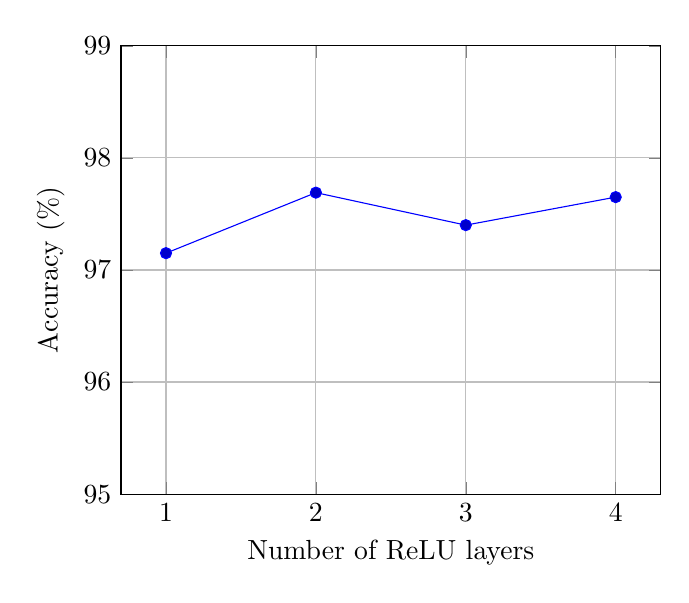
\begin{tikzpicture}
            \begin{axis}[
                    xlabel=Number of ReLU layers,
                    ylabel=Accuracy (\%),
                    ymin=95, ymax=99,
                    xtick={1, 2, 3, 4},
                    grid=major
                ]
                \addplot coordinates {
                        (1,97.14999794960022)
                        (2,97.68999814987183)
                        (3,97.39999771118164)
                        (4,97.64999747276306)
                    };
            \end{axis}
        \end{tikzpicture}
        \vspace{-0.1cm}
        \caption{Number of ReLU layers vs accuracy (128 neurons)}
        \label{figure:p21}
    \end{figure}

    As we can see above in \autoref{figure:p21}, increasing the number of ReLU layers (each with 128 neurons), does not consistently improve model accuracy.

    \subsection{Decreasing layer width}

    Here I want to experiment with decreasing layer width. This network starts with a 512 width ReLU layer, then one of width 256, then 128, then 64. For each iteration of this model, there is a 10 width softmax output layer.

    \pagebreak
    \begin{figure}[hb!]
        % \vspace{0.5\baselineskip}
        \centering
        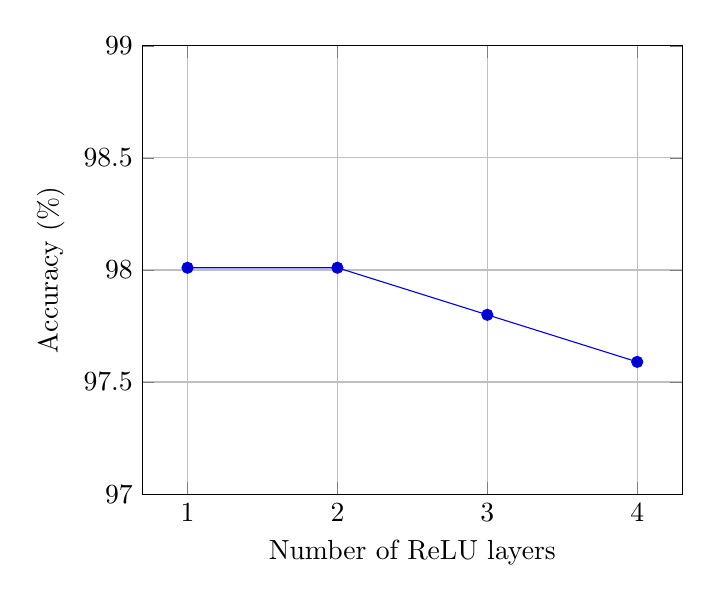
\begin{tikzpicture}
            \begin{axis}[
                    xlabel=Number of ReLU layers,
                    ylabel=Accuracy (\%),
                    ymin=97, ymax=99,
                    xtick={1, 2, 3, 4},
                    grid=major
                ]
                \addplot coordinates {
                        (1,98.00999760627747)
                        (2,98.00999760627747)
                        (3,97.79999852180481)
                        (4,97.58999943733215)
                    };
            \end{axis}
        \end{tikzpicture}
        \vspace{-0.1cm}
        \caption{Number of ReLU layers vs accuracy (narrowing width)}
        \label{figure:p22}
    \end{figure}

    Here we can see that the accuracy falls as I add more layers. As described above, I had the network narrowing as more and more layers were added. So in the above figure, the first point shows the performance of a $512 \rightarrow 10$ network, the second shows the accuracy of a $512 \rightarrow 256 \rightarrow 10$ network and so on. \\

    As is apparent from the above figure, a neural network with narrowing ReLU layers did not improve accuracy in this case.

\end{homeworkProblem}

\end{document}
